% ===================================================================== PARTE III
\chapter{Validación numérica}

Antes de creer un resultado hay que saber que el código calcula lo que dice. Las
pruebas automáticas (\archivo{tests/}) comparan el código con resultados conocidos de
antemano:

\begin{longtable}{p{0.45\textwidth}p{0.47\textwidth}}
\toprule
\textbf{Qué se verifica} & \textbf{Resultado} \\
\midrule
\endhead
RK4 contra la solución exacta $e^{Mt}x_0$ & error relativo $<10^{-6}$ \\
Conservación de $\sum_i x_i$ con difusión pura & variación $<10^{-10}$ \\
Tasa de recuperación $\alpha+D_0\lambda_2$ en redes simétricas & coincide al 1~\% \\
Kuramoto en red completa, Lorentz, $K=2$ & $r=0.7076$ simulado vs.\ $0.7071$ teórico \\
Eisenberg–Noe en un caso resuelto a mano & exacto \\
Dataset de la tarea 5 & idéntico bit a bit al regenerarlo \\
Motor multicapa con una capa vs.\ motor v1 & idénticos (error $<10^{-10}$) \\
Ruido: varianza estacionaria de Ornstein–Uhlenbeck $\sigma^2/2\alpha$ & coincide al 10~\% \\
Flujos estimados $\hat W$ vs.\ $W$ verdadero & error mediano $<5$~\% \\
Ritmos estimados desde pagos vs.\ verdaderos & error mediano $<5$~\% \\
Coherencia $\hat r_i$ estimada vs.\ $r_i$ del modelo & correlación $>0.8$ \\
Tasa de impago generada vs.\ objetivo & exacta por construcción (bisección) \\
Columnas \texttt{truth\_*} hacia un modelo & error inmediato \\
Cada página de la app & carga sin excepciones \\
\bottomrule
\end{longtable}

En total, 127 pruebas pasan (\texttt{uv run pytest}).

% ---------------------------------------------------------------------------
\chapter{Resultados de las tareas 1 a 5}

\section{Tarea 1: frontera de estabilidad $R=1$}
\begin{figure}[h]
\centering
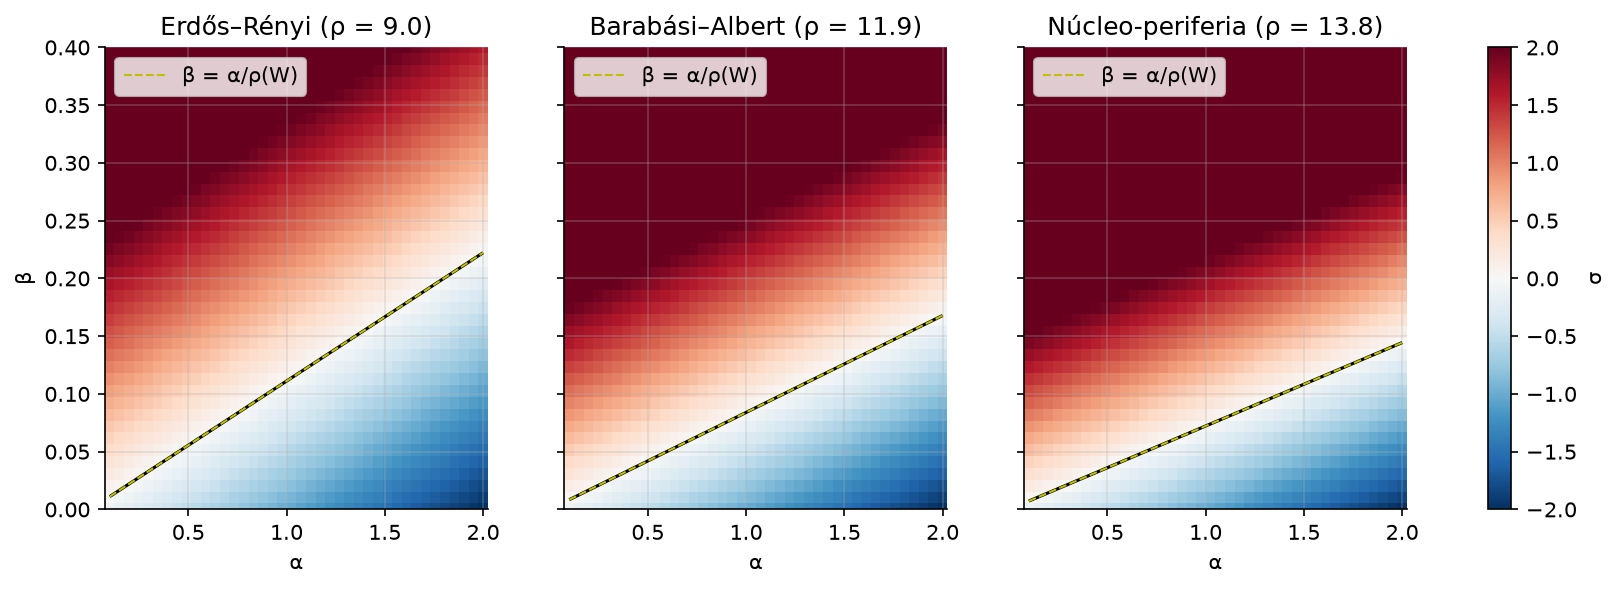
\includegraphics[width=\textwidth]{fase1_diagrama_alpha_beta.png}
\caption{Estabilidad en el plano $(\alpha,\beta)$ para las tres topologías. La línea
punteada es $\beta=\alpha/\rho(W)$, es decir $R=1$: por debajo la red amortigua (azul),
por encima amplifica (rojo). Las redes más concentradas (mayor $\rho$) se vuelven
inestables antes.}
\end{figure}
\begin{figure}[h]
\centering
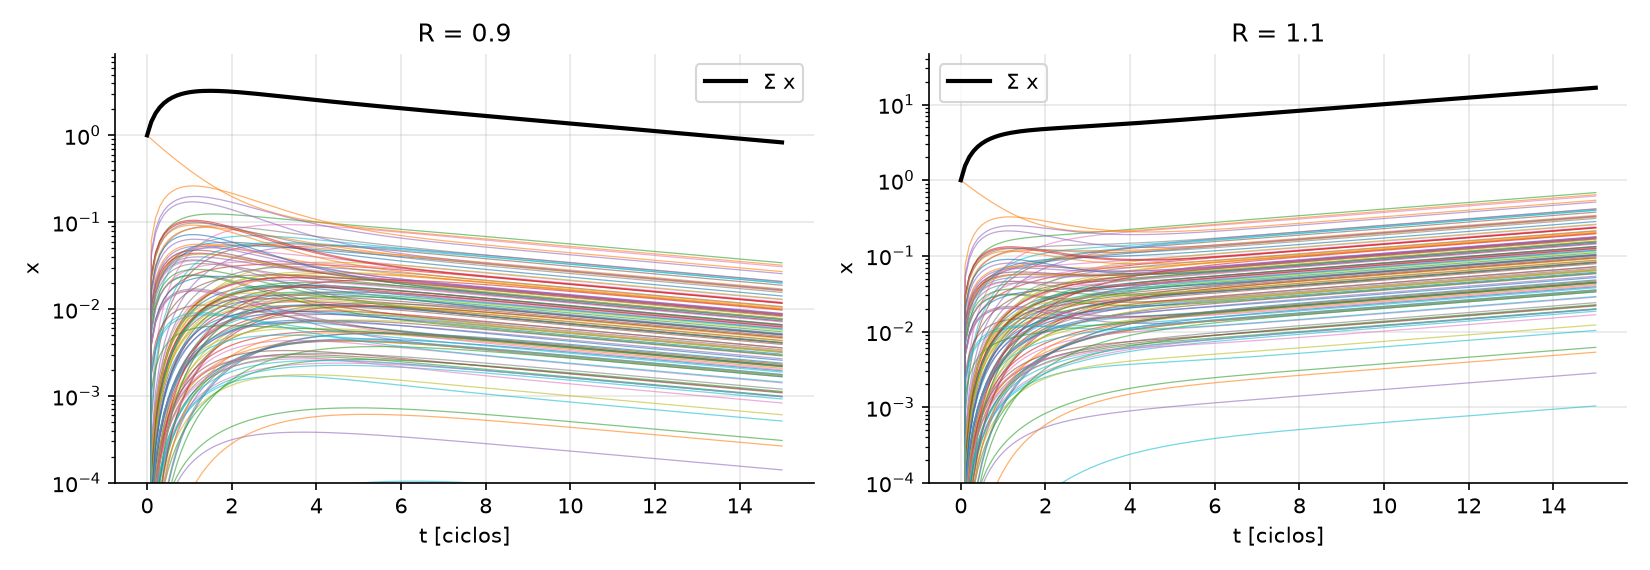
\includegraphics[width=0.9\textwidth]{fase1_trayectorias.png}
\caption{Déficit de cada entidad tras un choque con $R=0.9$ (se apaga) y $R=1.1$
(crece).}
\end{figure}

\section{Tarea 2: efecto estabilizador de la redistribución}
\begin{figure}[h]
\centering
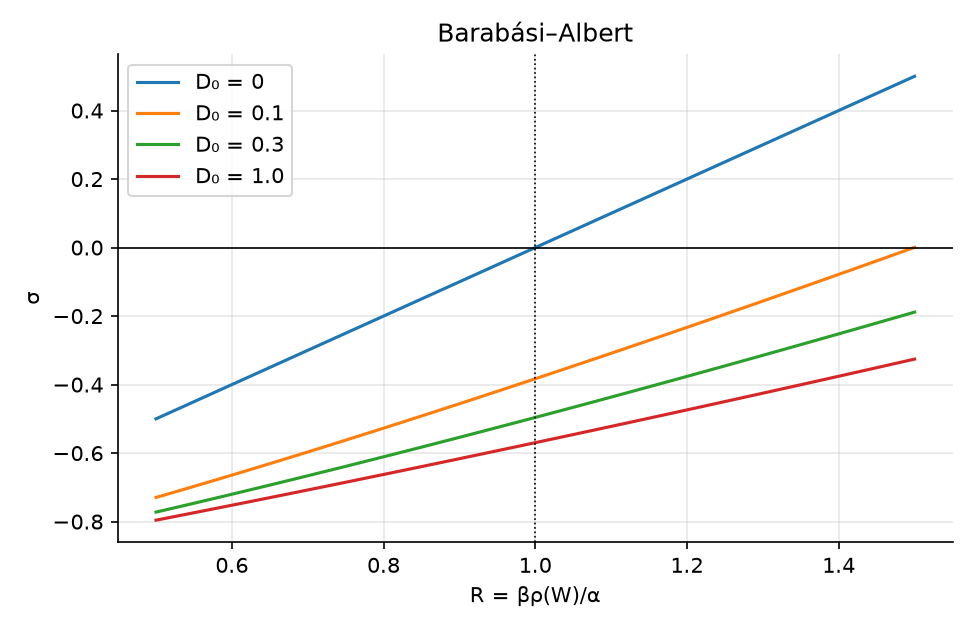
\includegraphics[width=0.48\textwidth]{fase2_D0_umbral.png}\hfill
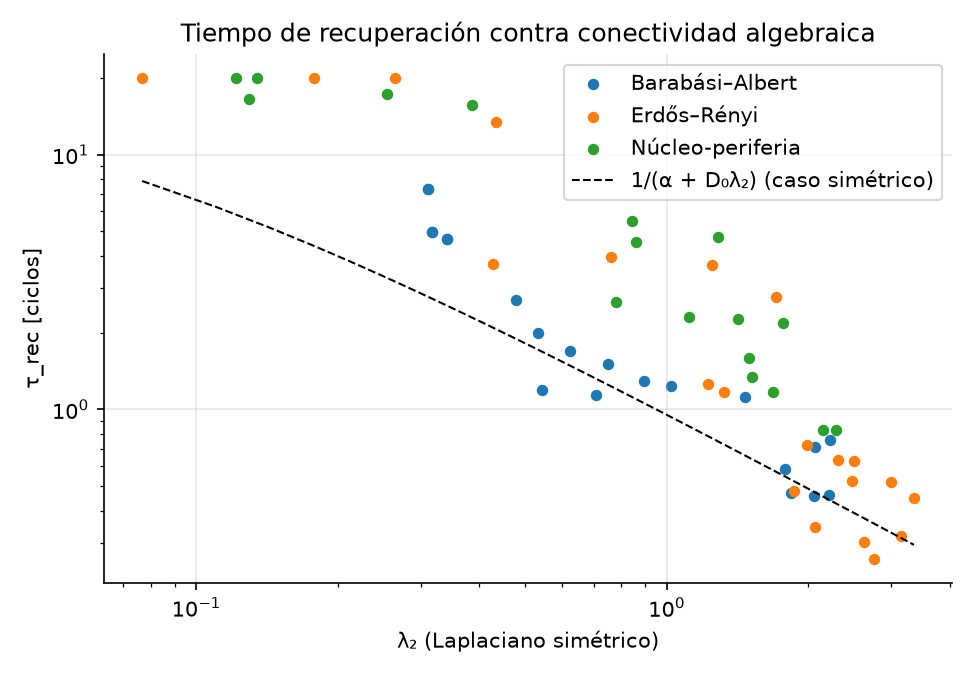
\includegraphics[width=0.48\textwidth]{fase2_tau_vs_lambda2.png}
\caption{Izquierda: con más redistribución $D_0$ la estabilidad $\sigma$ baja y la red
soporta valores de $R$ mayores que 1. Derecha: el tiempo de recuperación cae con la
conectividad algebraica $\lambda_2$; la línea es la predicción exacta del caso
simétrico.}
\end{figure}

\section{Tarea 3: transición de sincronización}
\begin{figure}[h]
\centering
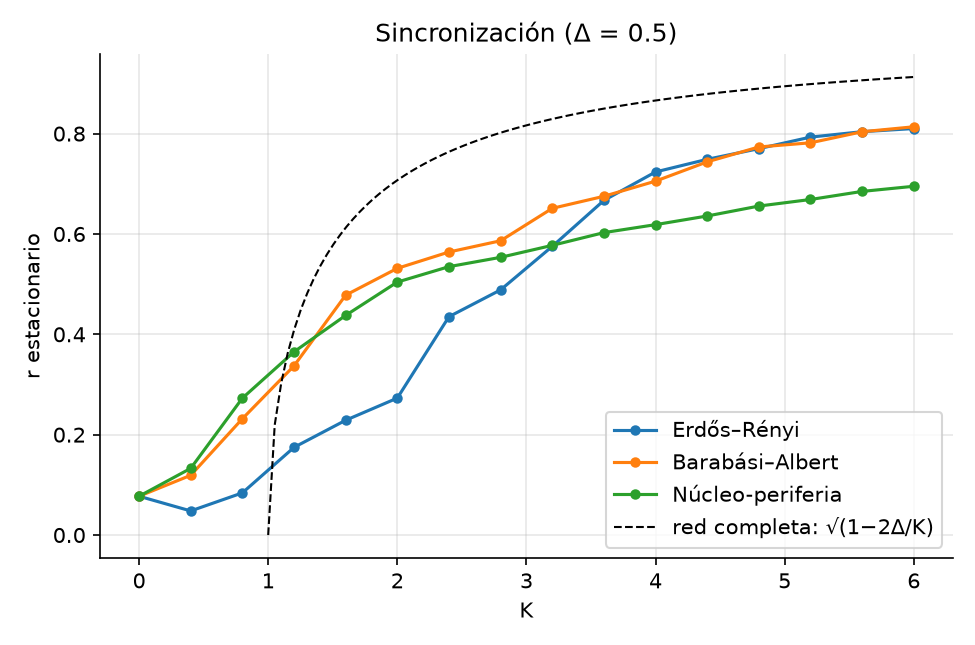
\includegraphics[width=0.6\textwidth]{fase3_r_vs_K.png}
\caption{Sincronía $r$ contra el acople $K$. La curva punteada es la solución
analítica de la red completa; las redes reales se sincronizan de forma más gradual.}
\end{figure}

\section{Tarea 4: cascadas de impago}
\begin{figure}[h]
\centering
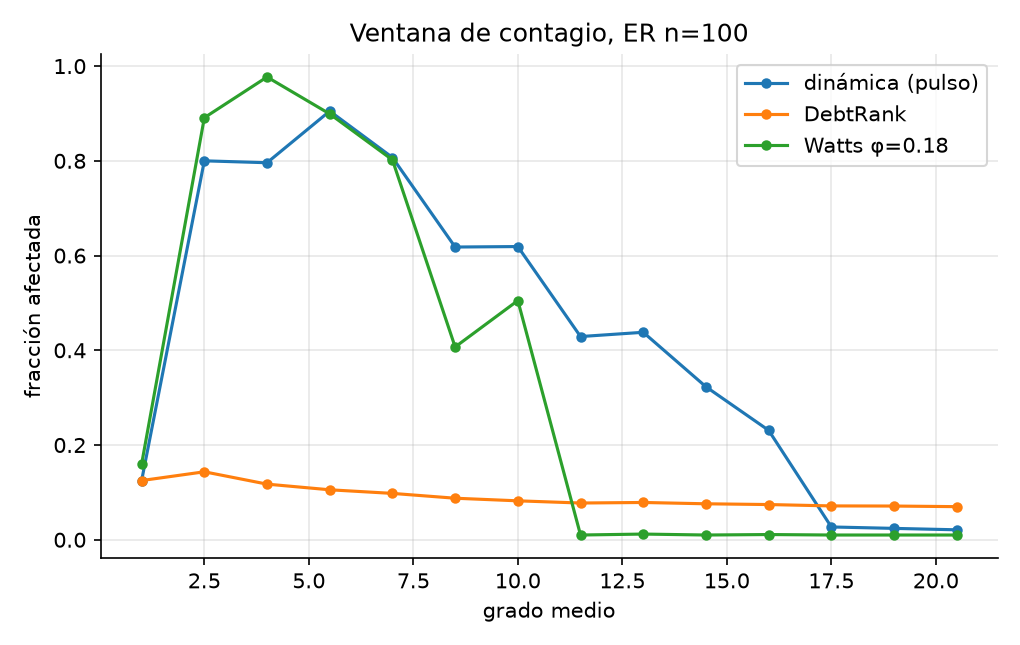
\includegraphics[width=0.55\textwidth]{fase4_ventana_contagio.png}
\caption{``Ventana de contagio'': fracción afectada contra el grado medio. Con pocas
conexiones el choque no se propaga; con muchas, cada entidad tiene suficientes
pagadores para absorber una pérdida; en medio, las cascadas son grandes. La dinámica
del proyecto, DebtRank y Watts muestran formas distintas.}
\end{figure}

\section{Tarea 5: desempeño predictivo}
\begin{center}
\begin{tabular}{llll}
\toprule
Modelo & Qué predice & Métricas (fuera de muestra) & Tiempo \\
\midrule
Regresión logística & colapso global & ROC-AUC 0.957 · PR-AUC 0.741 & 0.2 ms \\
XGBoost & colapso global & ROC-AUC \textbf{0.980} · PR-AUC \textbf{0.880} & 0.2 ms \\
XGBoost & cascada por entidad & $R^2$ 0.50 · Spearman intra-red 0.30 & 0.5 ms/red \\
GCN & cascada por entidad & $R^2$ \textbf{0.60} · Spearman intra-red 0.29 & 0.7 ms/red \\
\bottomrule
\end{tabular}
\end{center}
Una simulación cuesta $\sim$0.09~s por escenario: los modelos son unas $10^4$ veces más
rápidos. La PINN recupera $\gamma$ y $K$ con error menor al 1~\%, $\alpha$ al 7~\% y $\beta$
al 23~\% (el peor identificado, porque su efecto se confunde con el de $\alpha$).
\begin{limite}
Los modelos de entidades aciertan el \emph{nivel} de riesgo de una red, pero ordenan
solo moderadamente a las entidades dentro de ella (Spearman $\approx0.3$). Por eso la
app ofrece ``verificar con simulación''.
\end{limite}

% ---------------------------------------------------------------------------
\chapter{Resultados de la tarea 6}

\section{La comparación principal}
20 carteras por mundo (unas 39\,000 filas cliente-mundo por régimen), 6 meses de
observación y 12 de predicción, validación cruzada por mundo.

\begin{figure}[h]
\centering
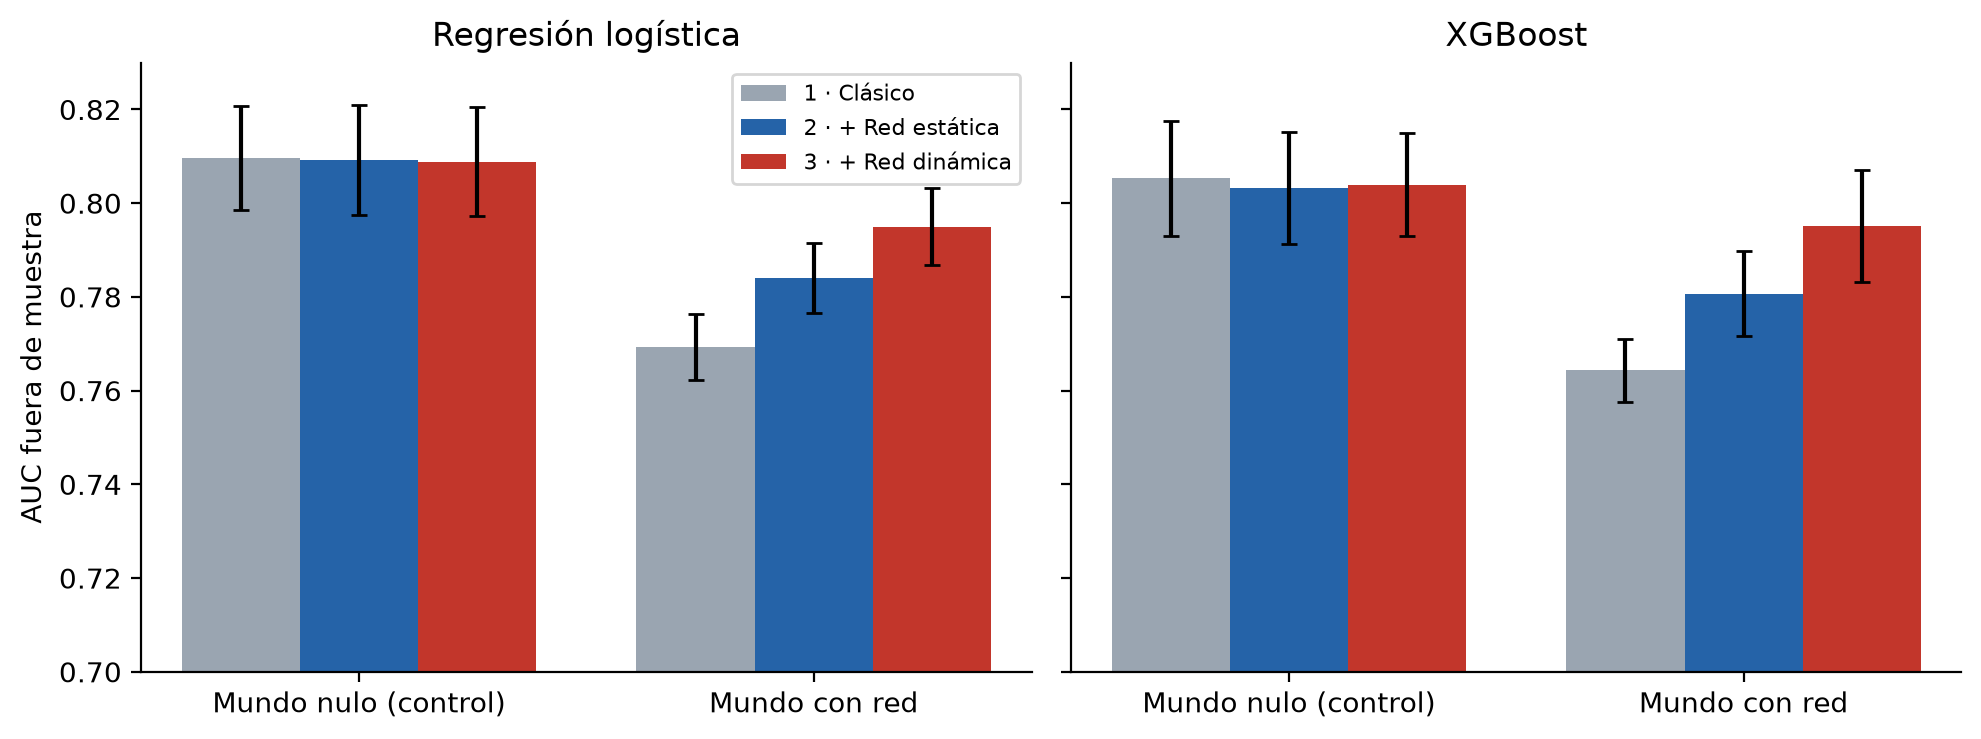
\includegraphics[width=\textwidth]{tarea6_auc_niveles.png}
\caption{AUC fuera de muestra por nivel de variables. En el mundo nulo los tres
niveles empatan; en el mundo con red cada nivel agrega información.}
\end{figure}

\begin{center}
\begin{tabular}{llccc}
\toprule
Mundo & Modelo & 1 · Clásico & 2 · + Red estática & 3 · + Red dinámica \\
\midrule
Nulo (control) & logística & 0.810 & 0.809 & 0.809 \\
Nulo (control) & XGBoost & 0.805 & 0.803 & 0.804 \\
Con red & logística & 0.769 & 0.784 & \textbf{0.795} \\
Con red & XGBoost & 0.764 & 0.781 & \textbf{0.795} \\
\bottomrule
\end{tabular}
\end{center}

\begin{figure}[h]
\centering
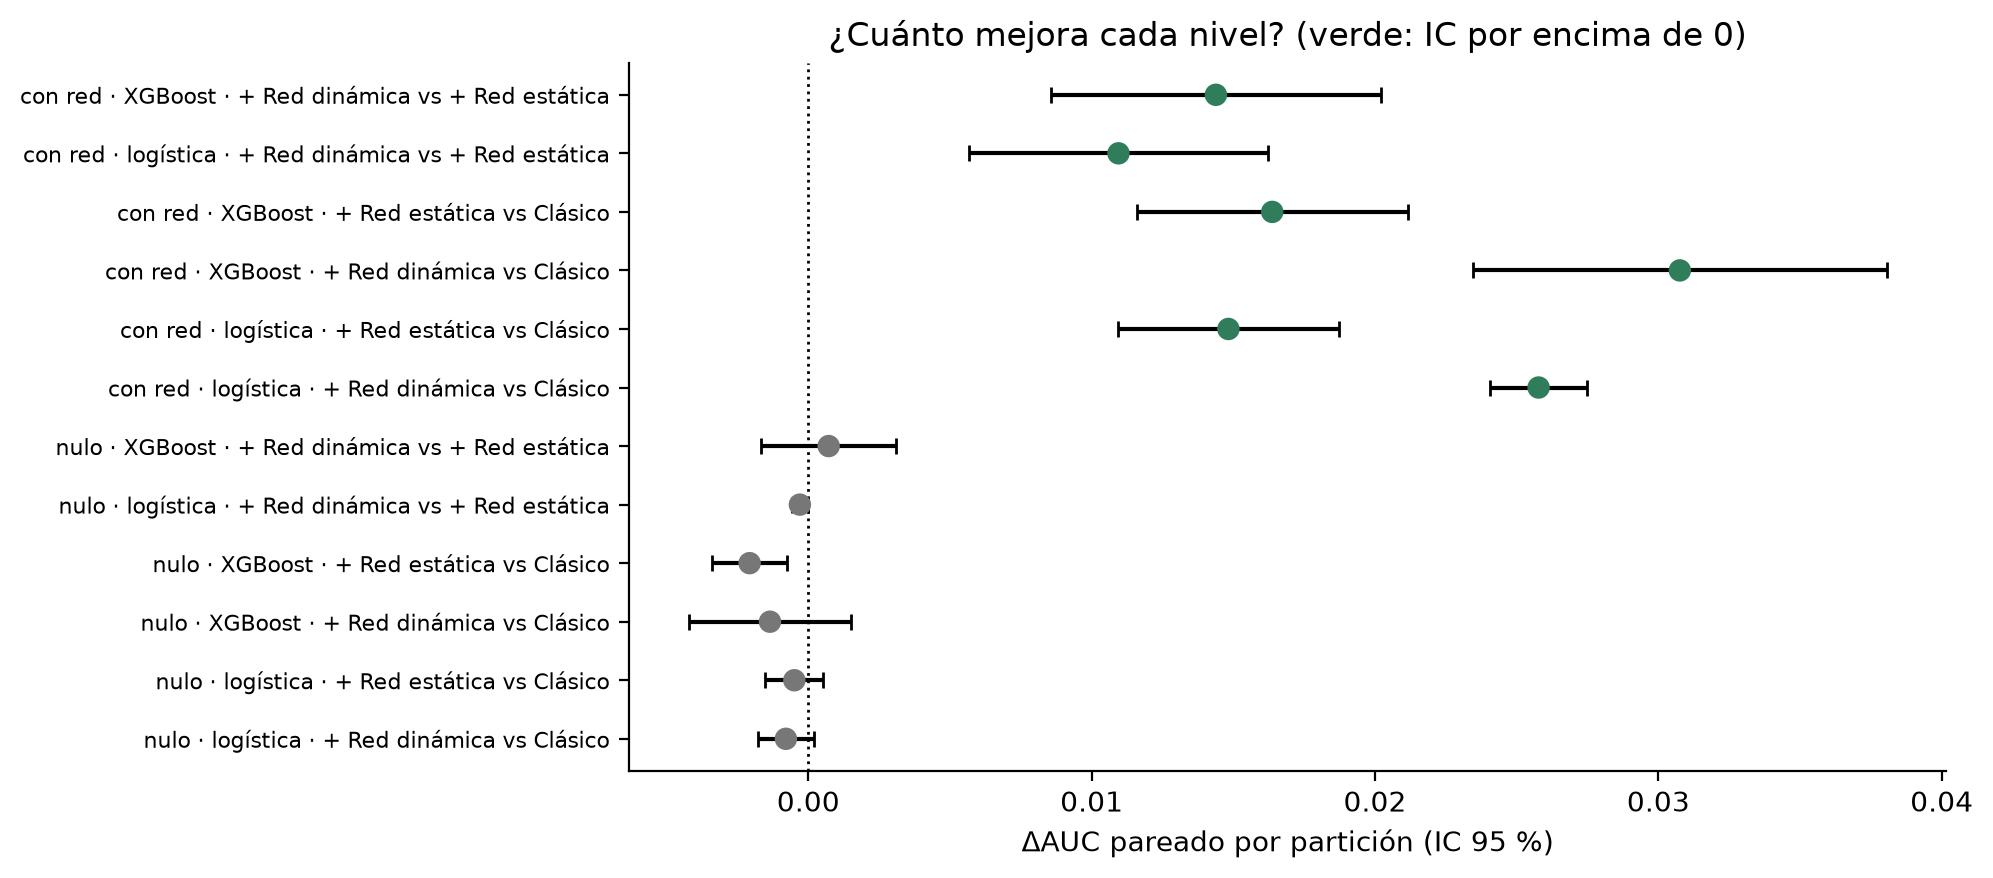
\includegraphics[width=0.92\textwidth]{tarea6_mejoras.png}
\caption{Mejoras pareadas de AUC con su intervalo de confianza del 95~\%. En verde, las
que están claramente por encima de cero.}
\end{figure}

\begin{clave}
En el mundo con red, la \textbf{dinámica mejora sobre la red estática}:
$\Delta\mathrm{AUC}=+0.011$ $[+0.006,+0.016]$ con logística y $+0.014$ $[+0.009,+0.020]$
con XGBoost, positiva en las 5 de 5 particiones; el PR-AUC sube de 0.277 (clásico) a
0.323. Frente al score clásico, el modelo completo gana $+0.026$ a $+0.031$. En el
\textbf{mundo nulo}, las mismas variables no aportan nada ($\Delta\mathrm{AUC}$ entre
$-0.002$ y $+0.001$): la mejora no es un artefacto ni una fuga.
\end{clave}

\section{Sincronización e impago}
\begin{figure}[h]
\centering
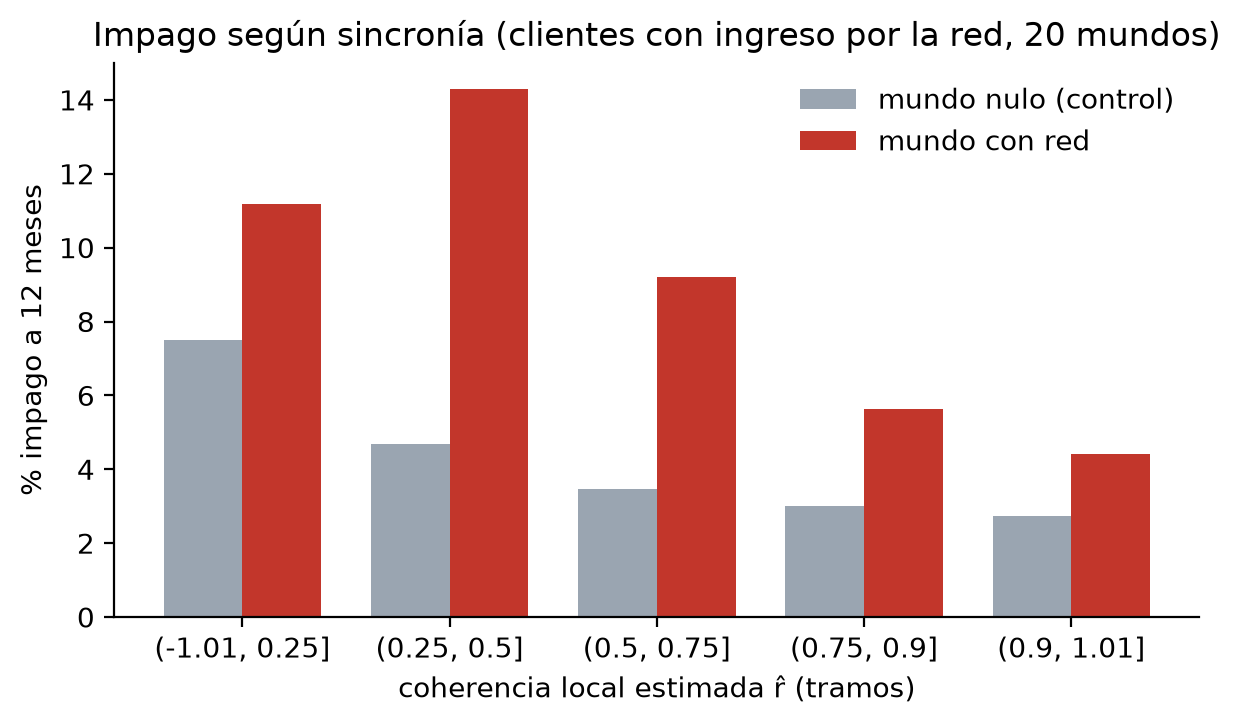
\includegraphics[width=0.8\textwidth]{tarea6_impago_por_r.png}
\caption{Tasa de impago por tramos de coherencia local estimada (solo clientes con
ingreso por la red). Con red, el impago pasa de 4.4~\% (bien sincronizados) a
11–14~\% (desincronizados).}
\end{figure}
\begin{nota}
En el mundo nulo también hay un gradiente (de 2.7~\% a 7.5~\%), pero se explica por
variables clásicas: los informales son más riesgosos y, a la vez, están menos
sincronizados. Por eso esta gráfica, sola, no prueba nada; la prueba es la
comparación de modelos con el control nulo.
\end{nota}

\section{Quiebra de un empleador}
\begin{figure}[h]
\centering
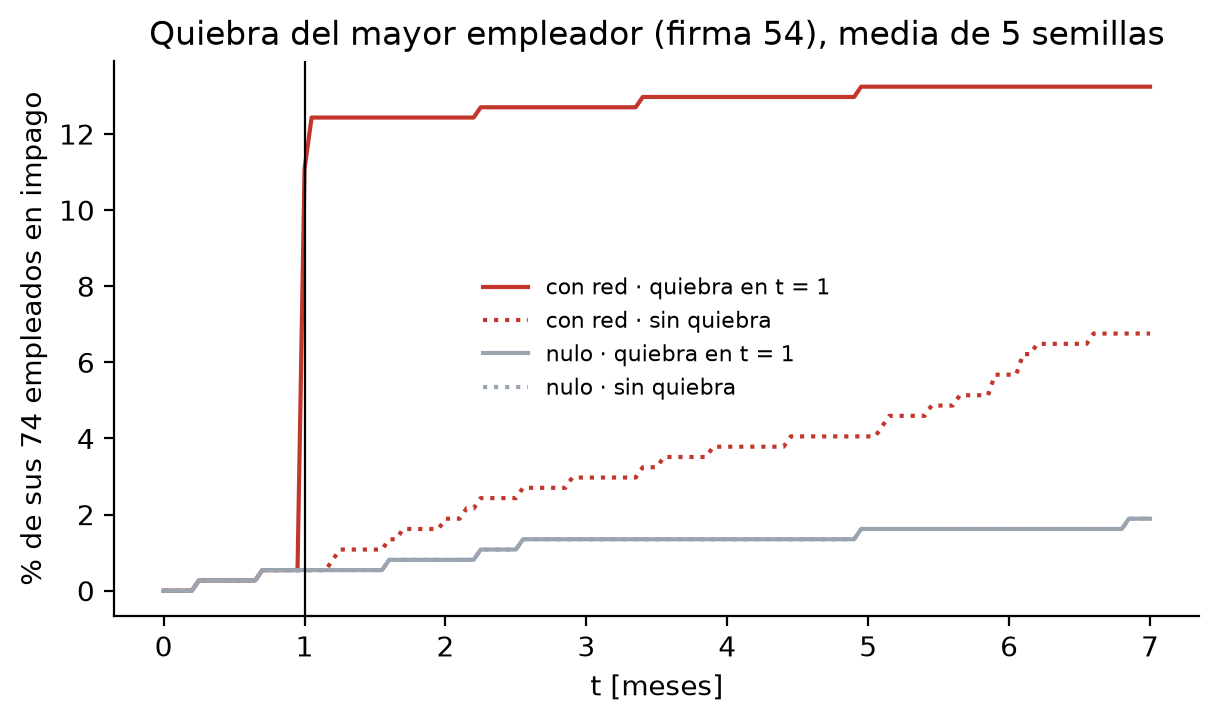
\includegraphics[width=0.8\textwidth]{tarea6_quiebra.png}
\caption{Empleados de la mayor firma de una cartera completa. Con red, la quiebra hace
caer al $\sim$12~\% de inmediato (contra $\sim$1~\% sin quiebra) y a los 6 meses llega a
13~\% (contra 7~\% sin quiebra, por la sola desincronización). En el mundo nulo la quiebra no cambia nada: la curva con y sin quiebra
coinciden.}
\end{figure}

\section{Interpretación y alcance}
\begin{itemize}
\item \textbf{Significa} que, si el mecanismo existe (los ingresos desfasados
generan estrés), entonces es \emph{detectable} solo con el registro de transacciones
que ya tiene un banco, y que aporta algo que la red estática no da.
\item \textbf{Significa} que el diseño experimental distingue señal de fuga: el
control nulo da cero.
\item \textbf{No significa} que el mecanismo exista en la realidad ni que la mejora
real sea de $+0.011$: los números dependen de parámetros ilustrativos ($\gamma$,
$K_\ell$, $\beta_\ell$\ldots).
\item \textbf{Siguiente paso} para convertirlo en evidencia: correr el mismo pipeline
(estimación, variables, evaluación) sobre datos reales anonimizados de una cartera.
El código ya está preparado: no usa nada que un banco no tenga.
\end{itemize}
